%!TEX root = project.tex

\chapter{About this project}
\paragraph{Abstract}
This project is about learning how to make a Open world game which means that the player is free to do what it wants and not just have to do the story that is given to them in the game, it is about letting the player go and look around the world that you have created and the AI that have been made from scratch. It is also about learning a new programming language as to the best of my limitations and to see what the language is capable of
\subsection{Source Code}
\url{https://github.com/Davidpurtill1101011/Project-Krantz-Mura}\\
\textbf{If you want to see any of the assets that I used please ask to see them by Emailing: davidpurtill29@gmail.com and I would be more than happy to do a call and talk about where they came from as they are not mine.}
\paragraph{Authors}
David Purtill, Programmer and Level Designer. 
\chapter{Introduction}
This project was decided on the objective of being able for my team partner and I to be able to go and learn a new language under our own initiative which is C++. With learning the language we also had to learn how to use the Unreal Engine 4 and to be able to use the editor to the full potential, and be able to make a somewhat functional game. This project is also set up to prepare us for a working environment such as being able to use \textbf{GitHub} to a proper standard and to be able to work with the remote GitHub online, and the also the local version of the remote repository. This should be able to have us learn over time on how to do pushes to remote via the command line and to be able to amend anything that goes wrong with the project and have a good amount of knowledge for the future.
\newline 
\newline
\textbf{Unreal Engine 4} is one of the top gaming editors/IDE there is to use for game development. The engine is so good that when it just has the bare minimum in it and without a character skin and just the basic UE4 the game looks superb. With setting up your game you are given the choice to pick between C++ and Blueprints these are both ways to make the game have functionality. We went with obvious choice and picked the C++ option. 
You are also given a few more options such as starter assets and this gives you some basic animations that you can use.
\newline
\newline
\textbf{C++} is used to just have all the player functionality such as
\newline Run,Walk,Jog,Crouch,Jump,Interact and do Punch Attacks all of these are setup/implemented in a .h file and then coded up in a .cpp file. This project was also had the idea of been able to use the \textbf{Unreal Engine 4} editor which itself can use a thing called Blueprints which are almost like code and C++ scripts where they can be wired together and kinda look like a wire-frame or a tree that is turned on its side, But as stated above we used the C++ route as it more efficient to use, that will be explained why in a chapter later.
\newline
\newline
\textbf{Objectives of the project.}
\begin{itemize}
    \item Player
    \item Artificial Intelligence(AI)
    \item Scene Editor
    \item Blender
\end{itemize}
The objective of the \textbf{Player} is to setup the inputs and basic movements for the user to be able to move around whilst playing the game, these inputs are the forward,back,left and right and a few more but that will be done below in the Tech review.
\newline
\newline
\textbf{Artificial Intelligence} is the non playable characters that are in the game but can be enemies and friendlies but for our game we just have enemies setup for the moment. The enemies can and will detect you if you enter a certain area this will go more in-depth in the tech review and how it was coded up.
\newline
\newline
\textbf{Scene Editor} this heading will talk about how the landscaping of the map is done and how the assets are added in and make the world look more realistic.
\newline\newline
\textbf{Blender} is a tool that is used to make assets and this is something that i had to learn on the fly while coding up somthing at the time and it was hard to find free assets for said object so i did some work in this, i will explain how i had to use this later.
\newline\newline
The list below is of the chapters that are going to describe how the project was done \\[0.2cm] \textbf{Chapters of the project.}
\begin{itemize}
    \item Methodology
    \item Technology Review
    \item System Design
    \item System Evaluation
\end{itemize}

\textbf{Methodology}
This chapter will go through about how we setup the project and the storyboards/story we had for the game. We will talk about the gantt chart with the sprints we had set up in that chart for what needed to be done. We also setup a kanban on Github to use for what was needed and what had to done and finished. All of these were very helpful for the project for me to follow and if needed we could add an issue to the Kanban and have both people to look at it.
\newline
\newline
\textbf{Technology Review} 
The Technology Review chapter will talk about all the Technologies that I myself had to use during the project such as Github, Unreal Engine 4(C++), Visual Studio 2019 \& Visual Studio Code and Blender. All of these were used to the best of my knowledge and that will be explained more in the chapter below. Out of all the tools that were listed above Blender proved to be the trickiest to learn.
\newline
\newline
\textbf{System Design}
will talk about how the whole of the system is actually used to make a game and how everything binds together for example: How the C++ code and be written to work back into the Unreal Engine and then be able to pick out an Animation montage and then work that to which way you want, this will be covered in the Tech Review and then talked how it bound together here.
\newline
\newline
\textbf{System Evaluation}
will look at how the project could have been different and how the overall project itself could have been done differently and better in some parts. This will also look at better ways of setting up the project to have a better work flow and better charts that can show the work being done over a sprint or two.
\chapter{Methodology}
My partner and I sat down and discussed which way would be the best to go about doing this project and what kind of methodologies we could use and how they would best suit our project. And the best ways we thought of going about it was using a Gantt chart which includes two sprints where sprint 1 was for semester one and sprint 2 was for semester 2 and was to run right up to the deadline date of hand up. Another idea was to use the Kanban on Github and it gave use that freedom to be able to learn more about Github and much needed experience which we needed and was very handy to keep track of what has been done and what needed to be worked on, it was also good to keep track if something had a bug in it and needed to be fixed at a later date.
\newline
\newline
We also scored the issues as to which was easiest to most difficult, Such as the level design would be something like a 1 or 2, player movement would be a 3 or 4 and the coding of the AI would be that much harder and be like a 5 and up. The scoring system was very good as something that was scored to difficult would be left till later and be added to the second sprint as you will see what was coded up in each sprint in the heading below.
 
\subsection{Gantt Chart}
We also sat down and made a gantt chart. The chart consisted of two sprints, where sprint 1 was between November and December and this was to focus on both the player functionality and the level design. And then sprint 2 was to add more player functionality and to do some more level design that was needed that either of use didn't get to do in sprint 1 and some added level design that was mentioned in some of the story we made up for the game. 

\subsection{Sprint 1}
The functionality of the player was the main focus here in this sprint as it was to do with the language C++ as this was the main part of the entire project that was being done. In sprint 1 the player movement was coded up, with just the basics such as player movement and such. The level design that I undertook was of a radio-tower that was on top of a hill that is to be set up between the prison area that my partner undertook and the village that was going to be added in on sprint 2.
\subsection{Sprint 2}
Was to add some more work to the landscaping and to add a small village that the player could go to anytime they wanted to as the game is an open world game. It was also to done up to add advanced movement to the player such as melee fighting and then maybe something with weapons. The other thing was to add AI that would be the enemy in the game and also attack/chase the enemy just to show that it works. Within this sprint I had started some code and then handed it off to my partner to finish off, which is something that could happen in a real life situation.

\subsection{Kanban Chart (Github)}
The Kanban chart was very useful, especially with it being on Github. The feature of it being on Github and the able to add issues that are created can be put straight into the backlog for the work to be done, And having this saved us time of having to use some other tool. Also with the Kanban being on github we could close issues and comment and work that we were doing by adding the issue number that was connected to each issue in the comment of the commit that was being made. 
\begin{figure}[H]
    \centering
    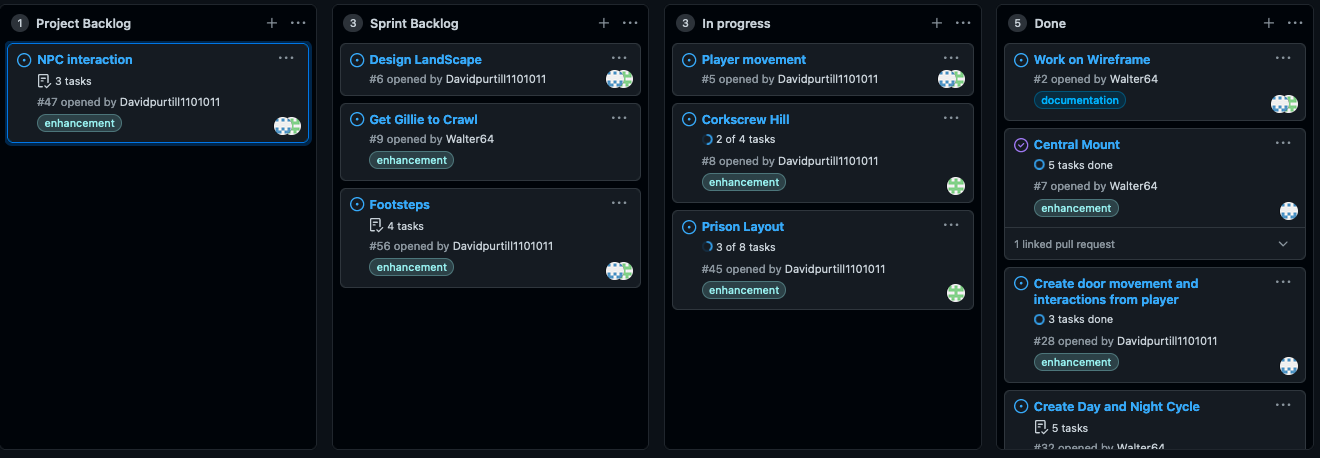
\includegraphics[scale=.3]{img/Kanban.png}
    \caption{Caption}
    \label{Kanbad chart}
\end{figure}

As you can see in the image above there is the Project Backlog where new or extra issues get put and then if they can be fitted into the Sprint Backlog we will add them in there. In Progress is where the current code is that we are working on is to be put and you can see that Player movement is issue \#5 and is in the In progress the longest of the longest as it was worked on over Sprints 1 and 2. And then the Done is where we put the issues that are finished but can be taken back out to add more work to or fix/refactor code.
\chapter{Technology Review}
\section{What is expected from Game Engine}
A Game engine should be able to do quite a bit for it to be a Game Engine and and Even more to be considered a good Game Engine
\begin{itemize}
    \item Should be able to make Both 2D and 3D games 
    \item Should be able to map key binds or inputs for keyboard and mouse, controller, touch pads, virtual reality sets and more.
    \item Animations editor.
    \item Sound editor.
    \item Scripts.
    \item AI(Artificial Intelligence).
    \item Documentation.
    \item Should be able to deploy to all platforms.
    \item Able to make multiplayer games.
    \item Cinematic Editor
    \item Landscape Designer
\end{itemize}
Most of the features of the list above are a given some game engines that are out there. But not all of them are in there altogether as for example that some game engines don't have a Cinematic Editor and will use Blender to do this which is used for making 3D models and also for making animated scenes that don't involve input from a user. But the most important thing that is need for any engine is that the documentation be the pinnacle of what it is all built on because if you have bad documentation how do you expect your game to get built. 
\subsection{The Right Engine}
\begin{figure}[H]
    \centering
    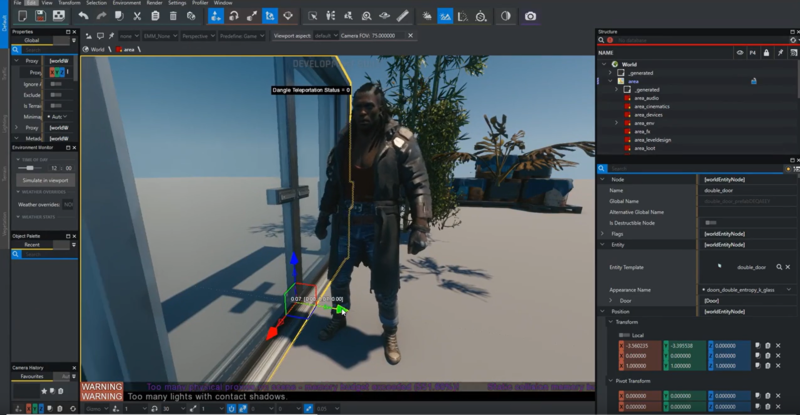
\includegraphics[scale=.5]{img/REDengine.png}
    \caption{REDEngine}
    \label{REDEngine}
\end{figure}
For making a game you need to pick the right engine for what you need to do and if you don't you could have a whole lot work done and then get to a dead end where the feature that your trying to add into the game cant be done as it not supported.
\newline
\newline
Something like this happened to a game that came out in 2020 it was supposed to be the greatest game that was going to be made in the last 20 odd years but the Developers/Owners had this great idea to make their own in house Game Engine called RedEngine this was supposed to be the next best thing but went down like a lead balloon which is not great when something like that happens. The reasoning behind this is that the engine wasn't great to handle the intense graphics of the game and the big thing was that there bad documentation for it and the devs were trying to fix bugs on the fly until they somehow or someone came across a fix for the bug.
\subsection{Unity}
\begin{figure}[H]
    \centering
    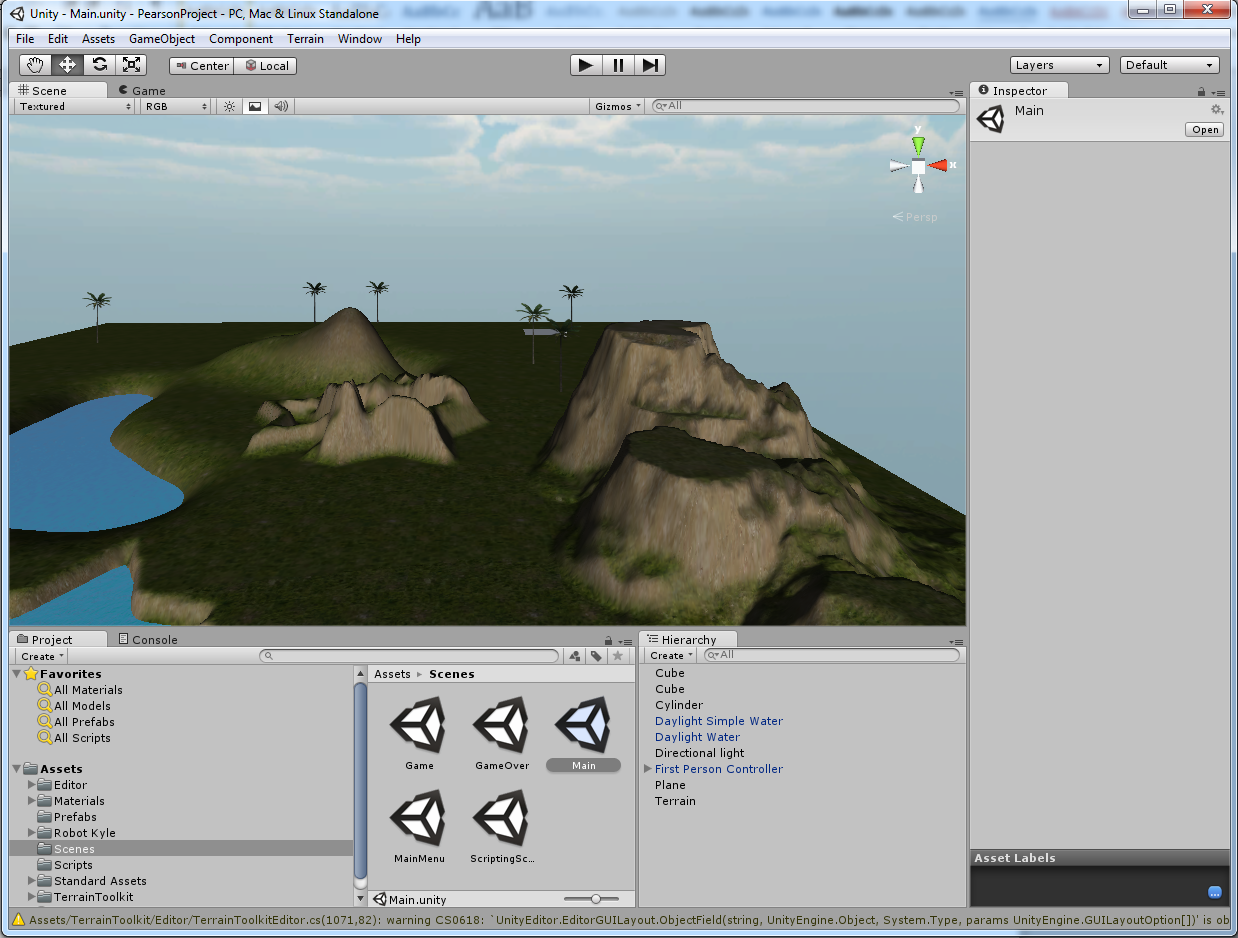
\includegraphics[scale=.3]{img/Unity.png}
    \caption{Unity Engine}
    \label{Unity}
\end{figure}
Unity is probably one of the most known game engines that is out there and is a very good and reliable engine. It has had numerous of next gen and ground breaking game built on it such as Escape from Tarkov which is setting the standards for first person shoots as it has everything from Ai to online multiplayer and excellent rendering of graphics. Rust is another game that is a mass multiplayer that was developed in 2013 and is constantly getting better 9 years later as the engine itself is constantly being updated and this lets the game engine kick it with the big dogs that are out there. With Unity you get all the bells and whistles that I mentioned at the start of this chapter which great for a person who is starting off and doesn't need to go and find a 3rd party solution to the problem as they can most likely find a guide or tutorial on how to do the exact thing they need as to where if it didn't it might put people off learning it and make them learn to use a different engine such as the likes of Unreal Engine which is the main competitor for unity and is doing a pretty good job of keeping up but with the latest update to the Unreal Engine being UE5 it is looking like it will be leaving quite a few of them in the dust as most companies that have their own inhouse systems are starting to jump ship to use UE5.
\subsection{Unreal Engine}
\begin{figure}[H]
    \centering
    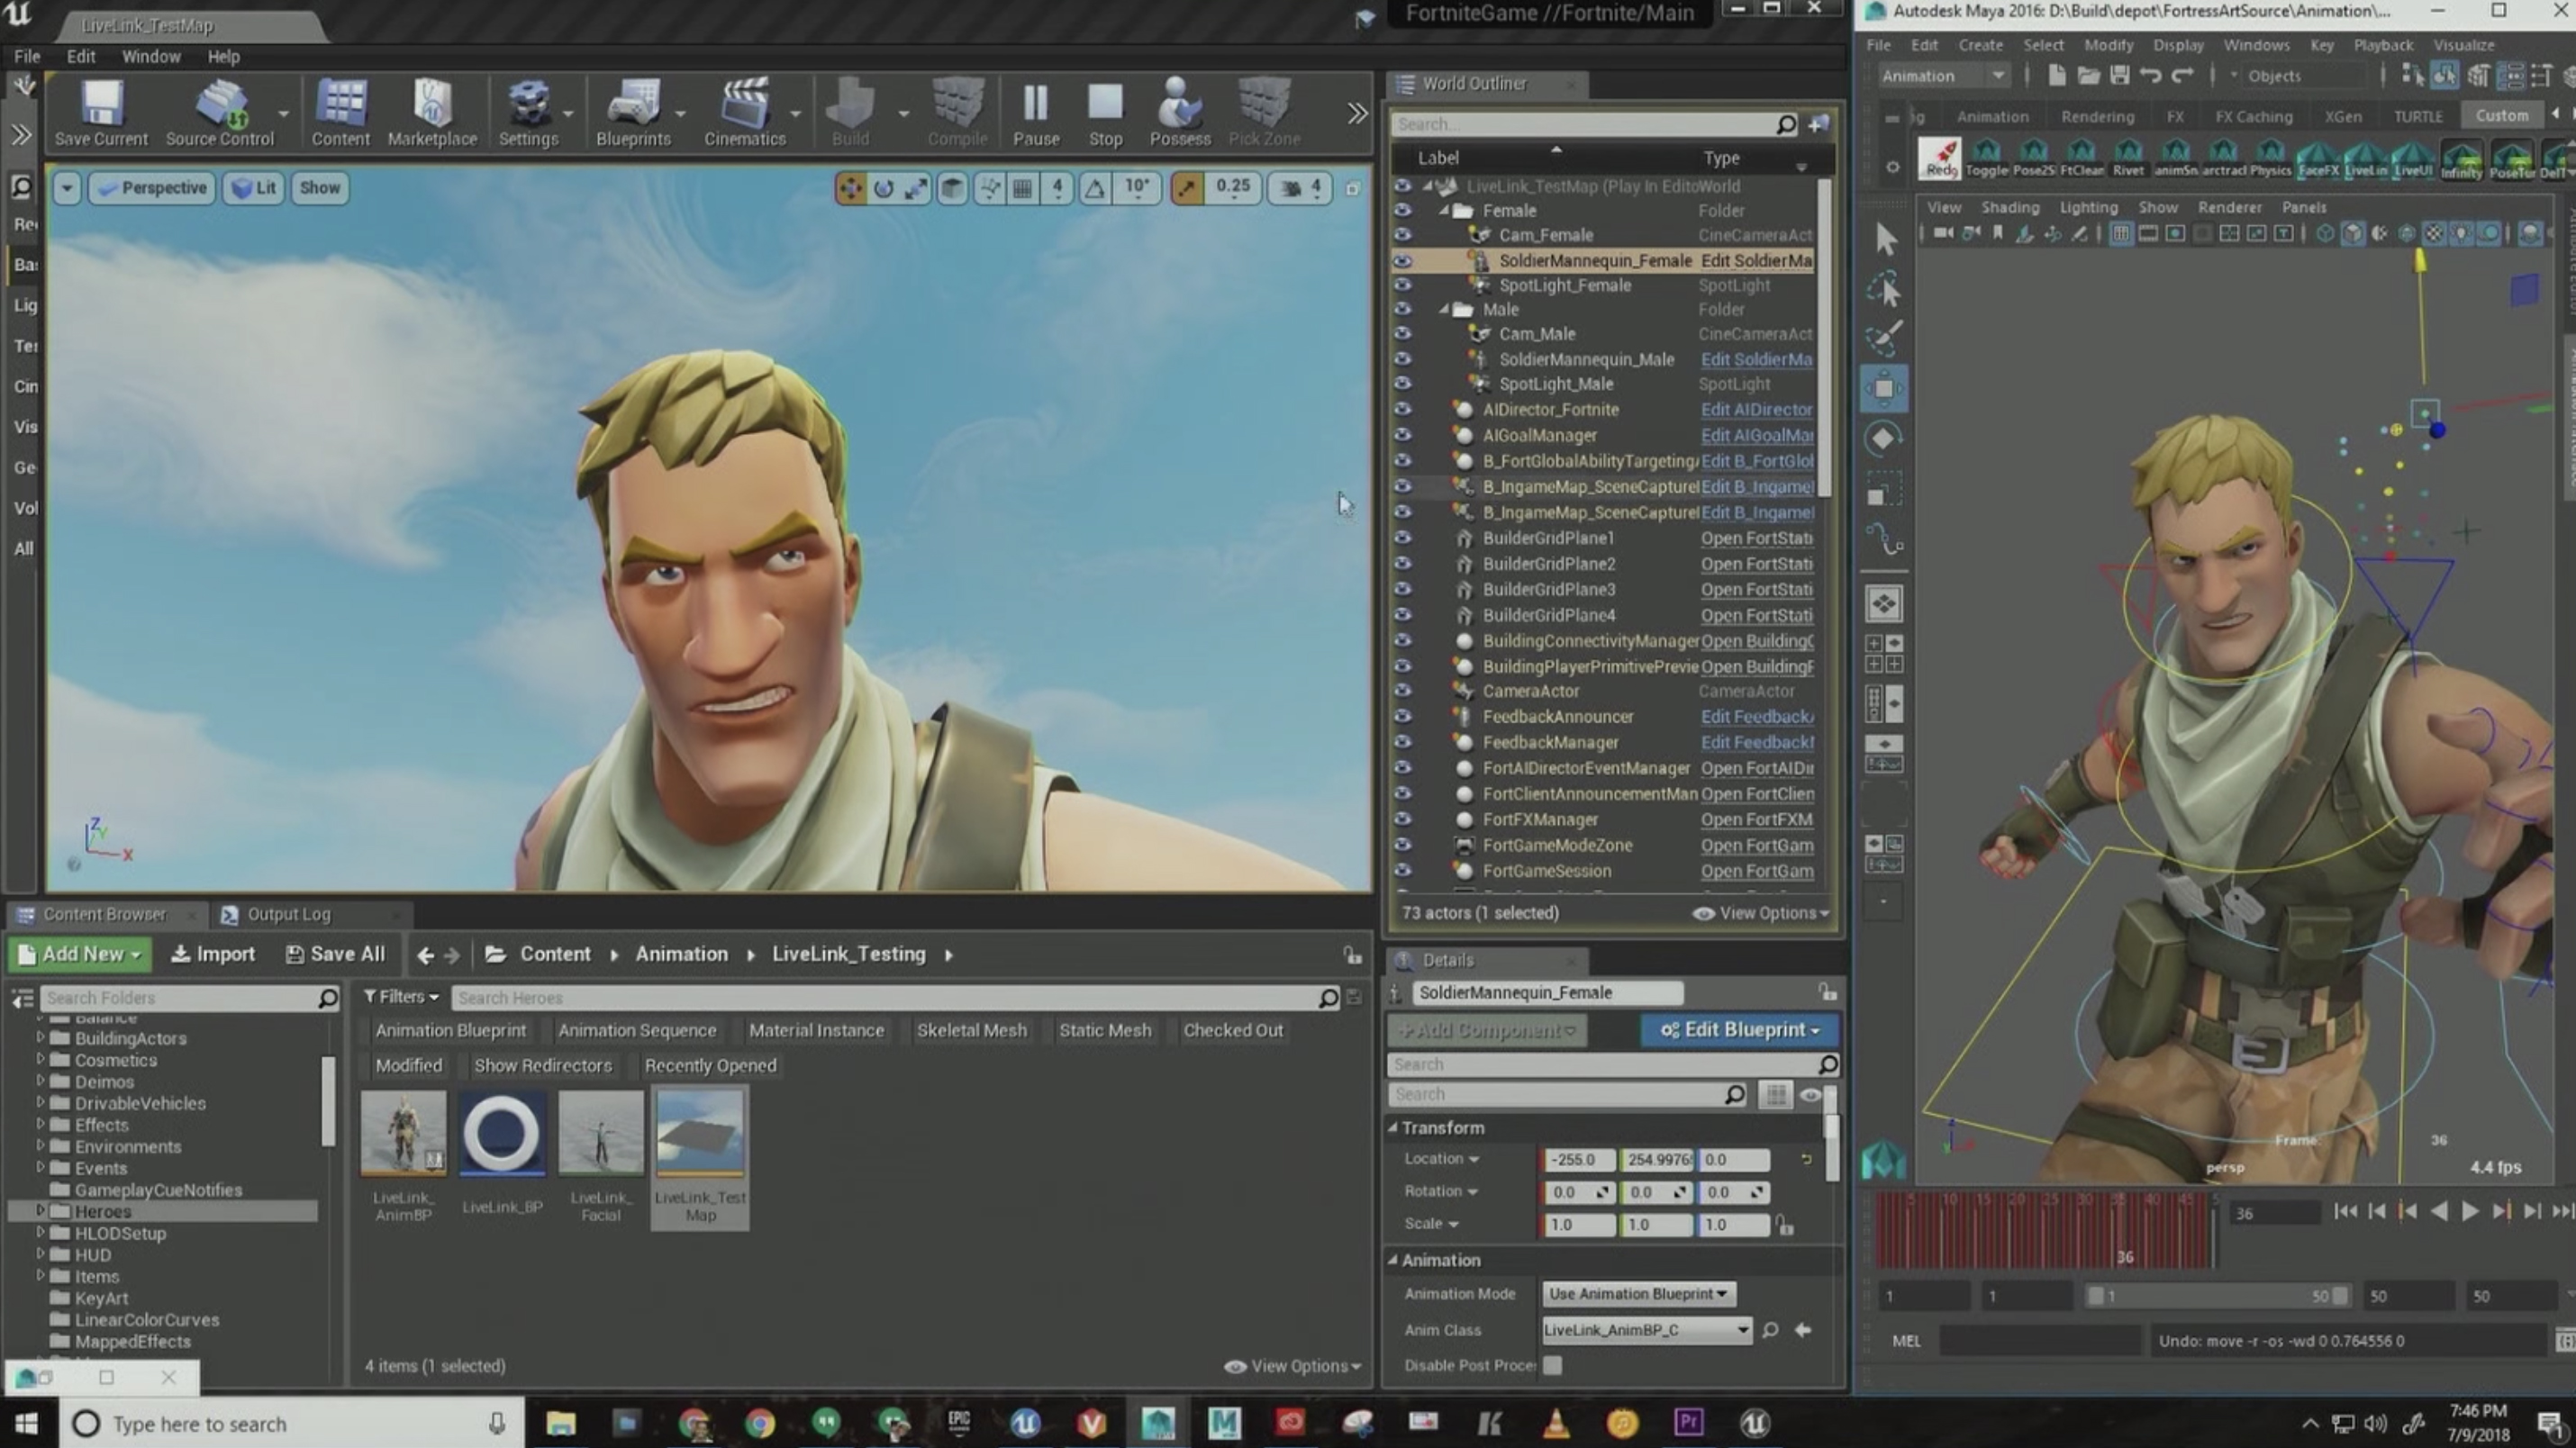
\includegraphics[scale=.3]{img/Unreal.jpg}
    \caption{BP Vars}
    \label{Unreal Engine}
\end{figure}
Unreal Engine has some of best cutting edge technology out there when it comes to game development and so much documentation out there you can go down a rabbit hole and having a tough time of getting back to where you started. Some of the games that are being developed on the unreal engine are out of this world on a graphics scale as well as the game play which is what every gamer wants, Hell Let Loose is a game that has some of the best graphics out there and some of the best game play out there by a country mile it and with just a team of 25 mixing between devs and level designers they are doing an excellent job. This is all down to the Engine being so user friendly and having so much out there in tutorials, courses and just YouTube videos. Unlike Unity Unreal has a way of making playable games without even having to use any C++ scripts and these are Blueprints.
\begin{figure}[H]
    \centering
    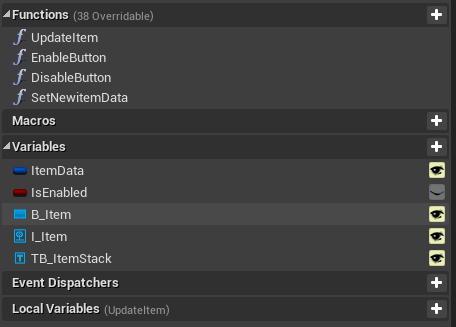
\includegraphics[scale=.7]{img/BlueprintVars.png}
    \caption{BP Vars}
    \label{Unreal Blueprints}
\end{figure}
These are essentially like circuit boards and all you have to do is wire everything together similar to how writing code, you have variables that are global for all other blueprints(functions) that all come together to make something functional or a playable game. For instance in the image above there are functions for Enabling and Disabling a button another to update the item that is in the players inventory and the last is to determine if the item is new or not and if so it will give it its own slot in the inventory. Blueprints can also be used with c++ and be blended together so they can be used to make a game this is something that most other open source engines dont have and this can make the game development process easier as it does not have be done by someone who knows how to write code.
\subsection{Unreal Engine using C++}
The reason behind using C++ as the scripting language is that C++ is one of the most powerful languages that is out there and has a direct line with using C as the header files and to declare all your variables, functions, properties and what libraries you are using and if you are importing or casting to another class in the .cpp(C++) file you need to tell it in the .h(Header(C)) file and because of this it makes the the development of the game incredibly reliable as it has been tried and tested over the years as such a good language but even better for using to develop games as it is so good at memory management, more control, very flexible and really good for optimization of game assets. If you were to use just purely C++ and no blueprints in your game you would have a game that would have no stutters and as to where if you were to use just blueprints your game would have quite a number of stutters as shown in the image below.
\begin{figure}[H]
    \centering
    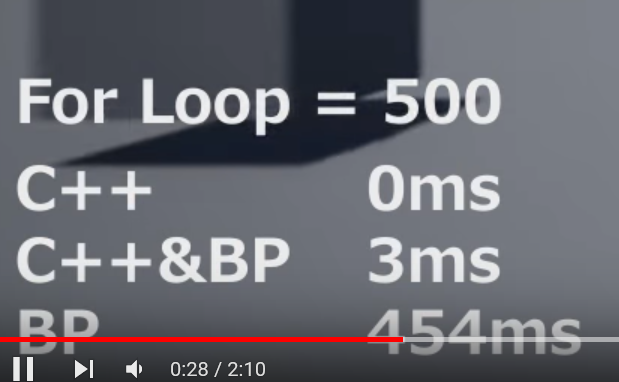
\includegraphics[scale=.6]{img/CPPvsBP.PNG}
    \caption{CPPvsBP}
    \label{Unreal Blueprints}
\end{figure}
As you can see in the screen grab from a video I found comparing  \href{https://www.youtube.com/watch?v=V707r4bkJOY&ab_channel=altalt}{C++ and Blueprints} going through a box and checking response times the for loop is set to 500 iterations and gets increased to 1000 this is where blueprints are not able to keep up as it just gives back an error. The only sign of struggle is when the loop is made to do 100000 iterations and C++ code just stops for 3 seconds and gets on with it. But these are all just testing the capabilities of the language more than anything. This is the reason as to why the language is so powerful and is used to create games.
\subsection{The benefits of Unreal Engine}
Unreal Engine or Epic who are the owners of the engine have set up the use of the engine to be completely free until the title you are working makes over €1 million euros or dollars that is when you have to pay royalties to Epic for the use of the engine. This idea is really good as it is very good for the likes of students, indie developers or even studios that are starting out and dont have the funding until they put the game to market and start making money off of it. This is where the choice was pretty simple as with having to use the best of everything you want in the Unity engine you need to pay a monthly fee of €150 and this is something that shouldn't be if your trying to get the best out of your game as to where you can get the full version of the Unreal Engine 5 for free and do as you like until you hit that €1 million mark and by then your hoping that the royalties are just pocket change to what you are making. On the epic store they do a free for a month where you can get assets that can be worth a fortune for completely free and they can be used for a project down the line or something that you are working on at the time, this is something that all others should follow as it lets people get creative seeing something in the store and it could then lead to something great.
\chapter{System Design}
\section{Unreal Engine 4 \& C++}
\subsection{Player}
The first thing that was done on the player was the basic movement/controls such as move forward, move back, move left and move right. All of the methods/functions are first defined in the .h file so to move forward the function that was created was \textbf{MoveForward()} even tho it is called moveforward it does both forward and backwards, And the function \textbf{MoveRight()} does the same for moving the player left and right. The code for moving the player left or right is the very same as \textbf{\ref{Movement}} but the only difference is that \textbf{EAxis::Y} makes the player move in that direction instead of forwards and back
\begin{figure}[H]
    \centering
    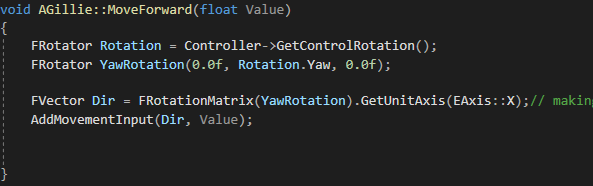
\includegraphics[scale=.9]{img/MoveCode.PNG}
    \caption{Player movement for forward and back.}
    \label{Movement}
\end{figure}
And this is then added to a function called \textbf{SetupPlayerInputComponent()} that is automatically created by the character class that you pick when you create the player character. And this is contains a parameter passed in called \textbf{UInputComponent* PlayerInputComponent} and has a Pointer represented by a \textbf{*} this is how you know you are using a pointer or not. The PlayerInputComponent then binds the function to the Unreal Engine which is where you set the buttons that are to be used.

\begin{figure}[H]
    \centering
    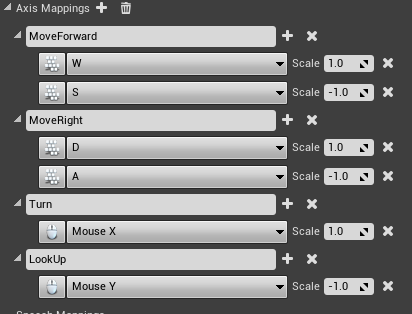
\includegraphics[scale=.5]{img/MovementInputs.PNG}
    \caption{Bindings for player movement}
    \label{Binding}
\end{figure}

As in the image \textbf{\ref{Binding}} you can see that W \& S are bound to the MoveForward and W has a positive 1.0 meaning that will make the player move in a forward motion and S has a negative number meaning the player will move backwards. And when binding these in in the C++ code you need to have the same exact name as what is used in the axis mapping or it will not work and this is something that will be easily be missed when your player wont or cant move forward for you.

\begin{figure}[H]
    \centering
    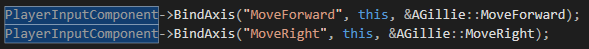
\includegraphics[scale=.9]{img/Mappings.PNG}
    \caption{Setting the function to the binding}
    \label{Mappings}
\end{figure}

With the image above you can see that "MoveForward" and "MoveRight" are both set to the MoveRight() and MoveForward() functions and are then bound to the input buttons that move the players in the directions they are set to. 
\newline
\newline
The next thing that was done on the player was to add a camera that would give a third person perspective. This style of camera would let you look over the players shoulder and be able to see a lot more of the game and lets the user enjoy the scenery that little bit more as you can get to take it all in.
But the coding up of this there had to be a USpringArmComponent* added to the player character and this acts almost like a boom for a camera and then you attach a UCameraComponent* to it which is the camera itself and this is controlled by the mouse and also is used to point the player in the right direction, look at \ref{Camera} to see how this was done.
\begin{figure}[H]
    \centering
    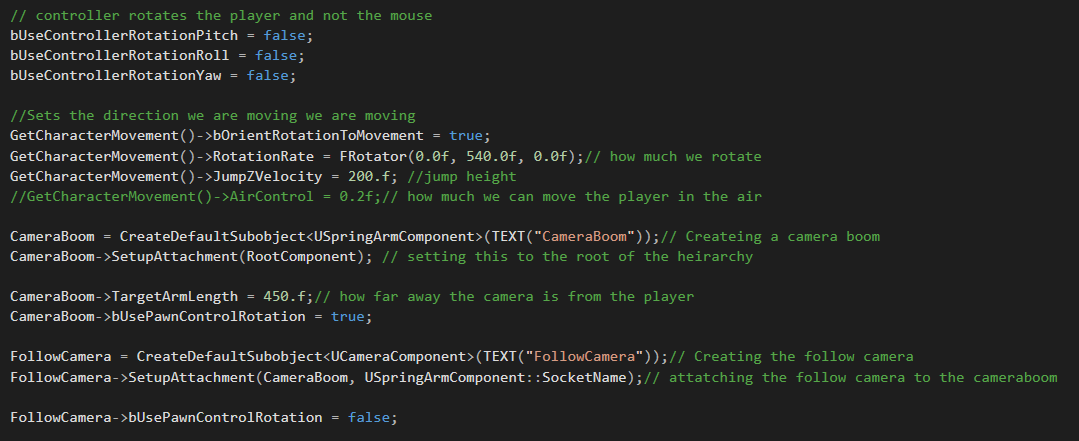
\includegraphics[scale=.5]{img/CameraSetup.PNG}
    \caption{Code for using the camera.}
    \label{Camera}
\end{figure}
After getting the player to do some basic movements and setting up the camera movement. The movement for Jumping and Crouching were then setup where Jumping is already in the Engine itself it just needs an variable to be added in this piece of code \textbf{GetCharacterMovement()->JumpZVelocity = 200.f;}, This line of code lets us add how high the player can jump and if it isn't ever initialized or set to 0 the player will never be able to jump even if it is bound to a button. 
\newline
\newline
For the crouching there had to be animations set-up and this is where the basic animations that you get from adding the starter pack stuff and the animations that are used are from there. So for setting up the crouch animations there had to be a new animation made called \textbf{BS\_Crouch} and then there was two animations taken from the assets called \textbf{MCO Mocap Basics}. These animations are for sitting still and one for moving while in the crouched position, so when you move forward the crouched walking animation will be set to active \ref{Crouch}.
\begin{figure}[H]
    \centering
    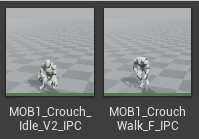
\includegraphics[scale=.8]{img/Crouch.PNG}
    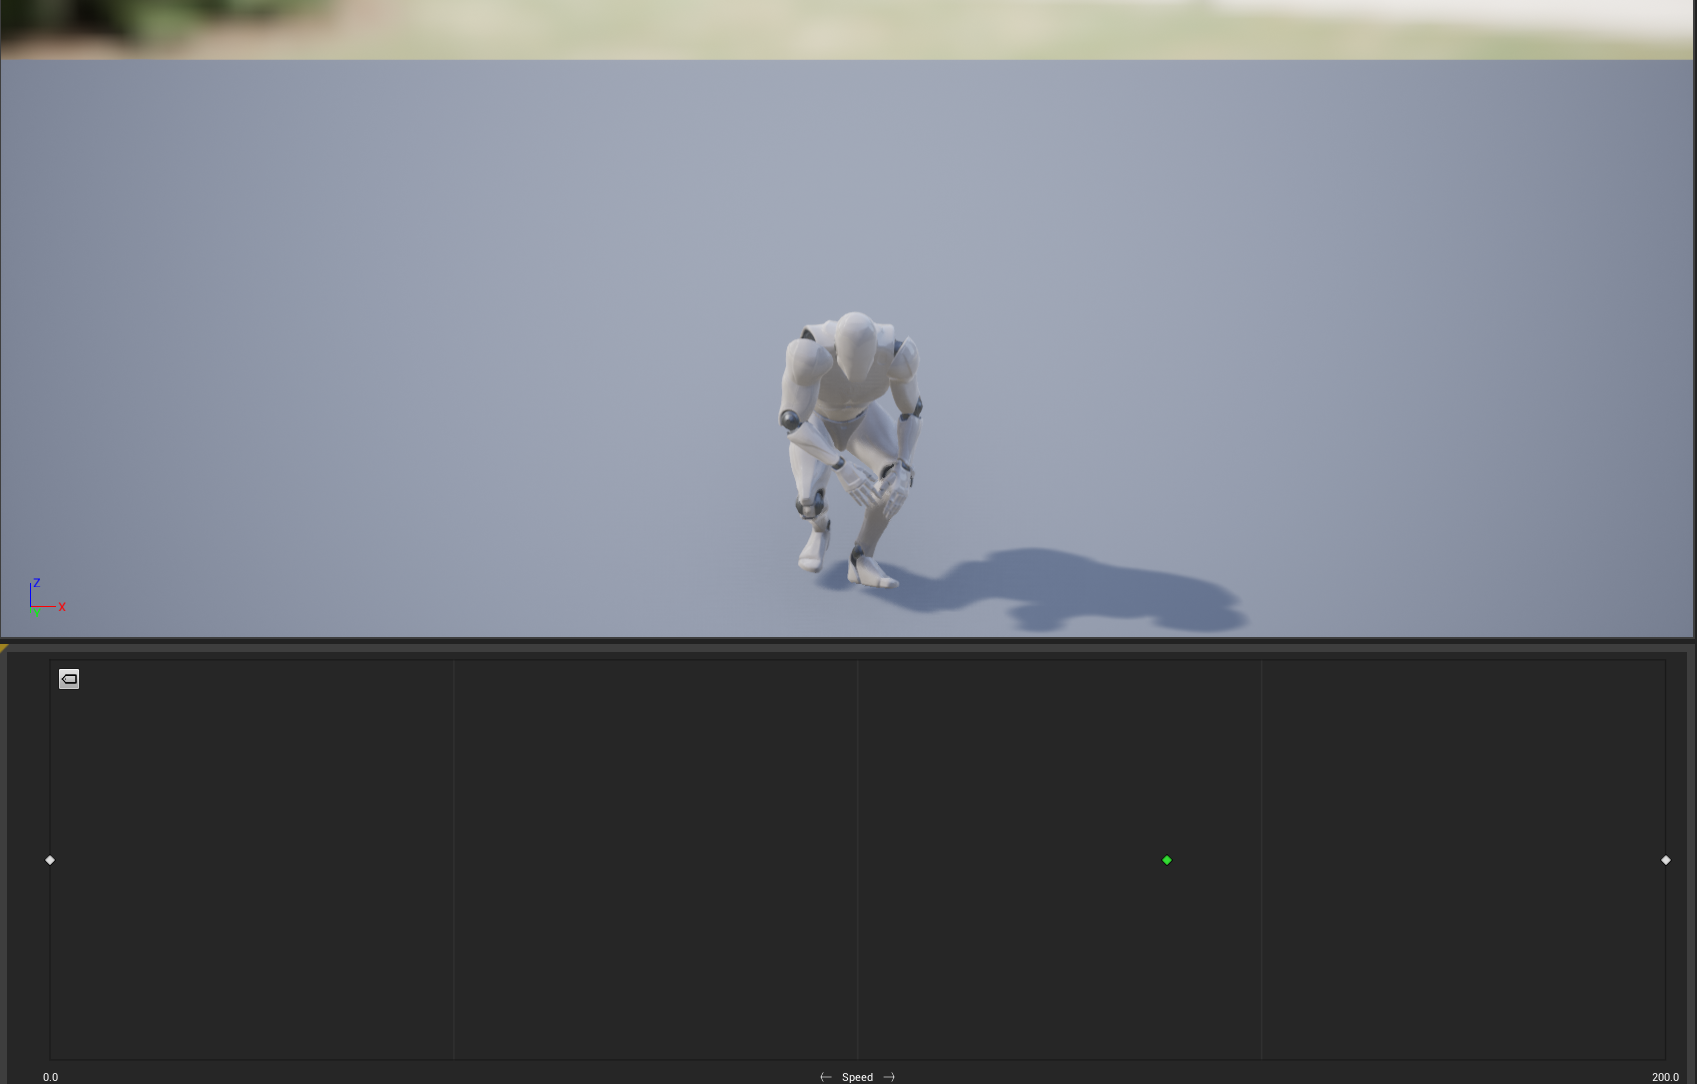
\includegraphics[scale=.15]{img/Crouch_BS.PNG}
    \caption{Animations for crouching}
    \label{Crouch}
\end{figure}
So after the BS\_Crouch animation was initialized the two animations that are in the image \ref{Crouch} are added in to that and then they are set to where if you are at idle the animation will do noting and that is at the most left part of the slider and then when you move that is at the most right of the slider and this then is setup in an animation blueprint \ref{Crouch}. The animation is then fully set up in the animation blueprint where there is a variable in there that is called isCrouching and this needs to be set to true when the player presses the left control button. And you can see this is the image \ref{Crouch_BP}
\begin{figure}[H]
    \centering
    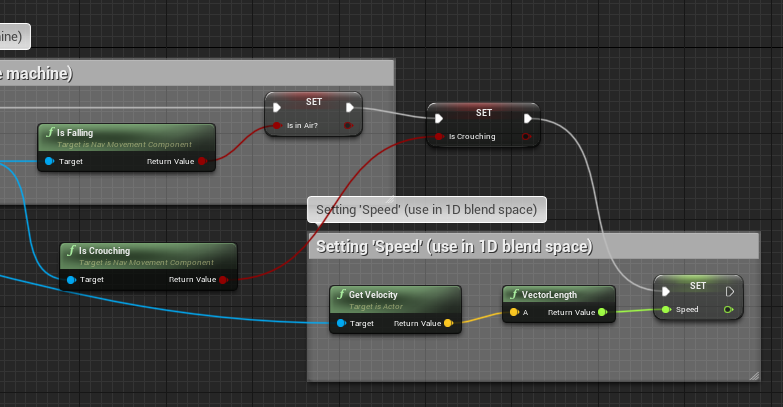
\includegraphics[scale=.6]{img/Crouch_BP.PNG}
    \caption{Animation Blueprint}
    \label{Crouch_BP}
\end{figure}
After doing the crouching animations I swapped most of the other animations such as walking,jogging and spiriting to look more realistic as they didn't look as rigid and looked like the player was actually would go from a jog to a sprint and to a walk. When all those animations were changed there was three  animations added for being idle where they would play randomly every time the player stopped moving and wouldn't play them in a loop as then it would get boring. And adding these idle animations would add some character to the player instead of being stood still and not moving.
\begin{figure}[H]
    \centering
    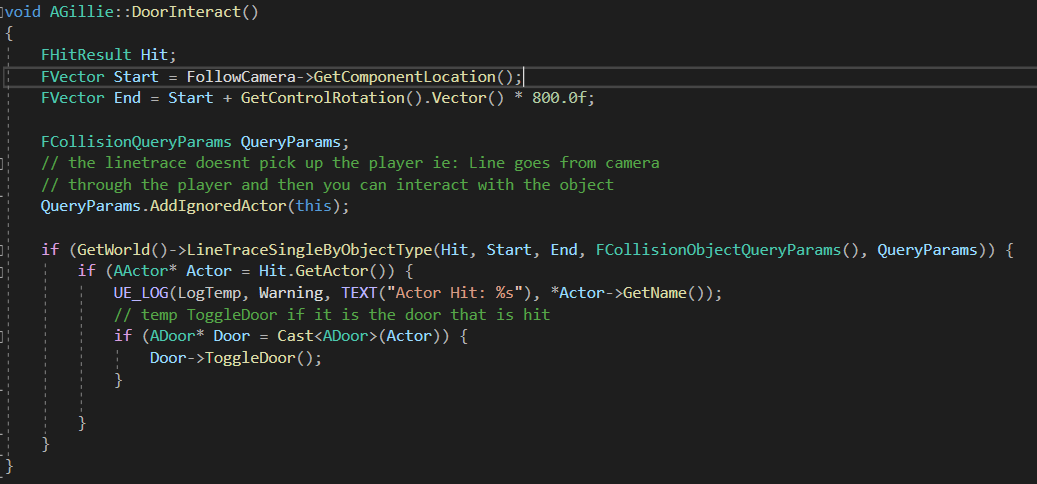
\includegraphics[scale=.6]{img/DoorInteract.PNG}
    \caption{Animation Blueprint}
    \label{Crouch_BP}
\end{figure}
After I got the player moving around. I setup an interaction with doors that can be opened and closed when the player was at a certain distance from it and pressed E on the keyboard this keystroke was assigned the name Interact and this could then be in turn be used for anything else that could be interacted with. And how I determined the distance from the player to the door was by adding a thing called a Line-trace which makes an invisible line from the players head to a certain distance you want them to interact with what you have setup. So if the player was set to be able to interact with door at 500.f then the line is cut to that size and when it touches the door you are able to open and close it. But if you open the door the Line-trace will not be touching the door and will not let you close the door until you are looking at it.
\newline
\newline
Setting this up proved to be a little tricky as some of the Documentation that is out there seemed to be a little out dated and the libraries that were needed from the documentation were in different set of libraries which I found out from watching a video on how to make the door and set up the Line-trace.
\newline
\newline
The player has a second Interact function that lets them pick up items that are in the world. These items are the likes of Health items and food items. This function is setup slightly different to how the door interact is wrote up. The ItemInteract uses a Interface that has a Interact function that takes a parameter of the player which makes the code to be more flexible as it is used for the Item class and when called in there it lets the player to pick up the item and destroys the object from the world and moves it into the players inventory.
\newline
\newline
\begin{figure}[H]
    \centering
    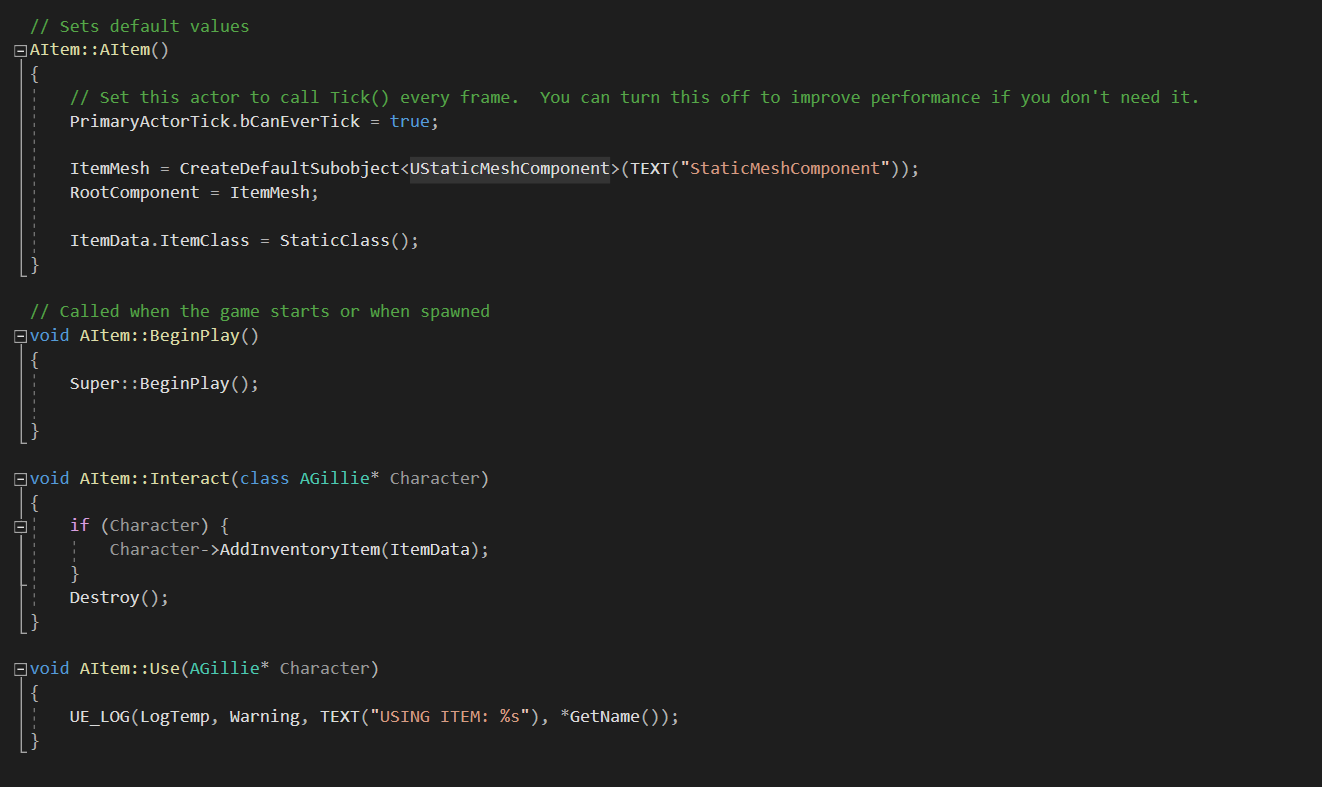
\includegraphics[scale=.3]{img/Item.PNG}
    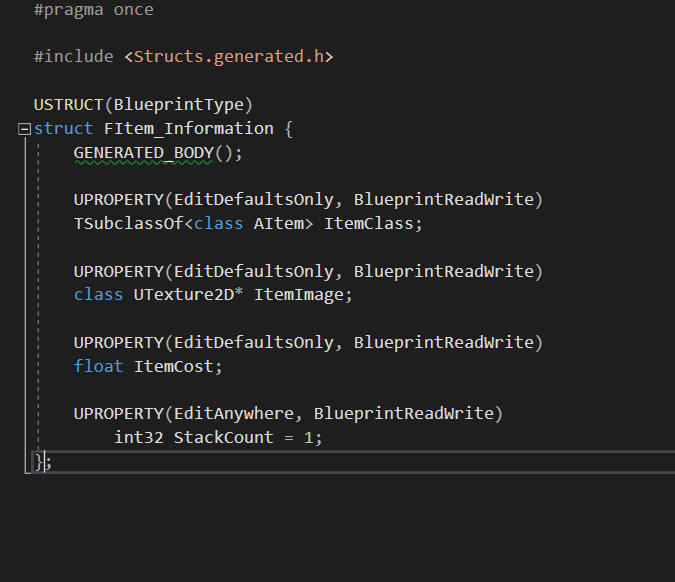
\includegraphics[scale=.5]{img/Struct.PNG}
    \caption{Item and Struct}
    \label{Item and Struct}
\end{figure}
The items health and food are both derived from a parent class called Item. The item class takes in a \textbf{UStaticMeshComponent} that can be set to whatever you want it to look like in the world. The item class also takes from header file that is \textbf{Structs} which has all the details such as what the image of the item,cost,what kind of class it can be assigned from the derived item classes that have been made from it. It also has an int32 called Stackcount that tracks the amount of each item you have in the inventory. So if you have 10 Health items it wont take up 10 slots but it will just increment the Stackcount and when it is then back to 0 it will remove it from the item from the player Inventory.
\subsection{Player Inventory}
With setting up the Player Inventory this was done with widgets called Interface,Inventory,IventoryItem and PlayerHUD. These all combine to add a cross-hair to the screen and is assigned to open the player inventory by using \textbf{I}. The image below is how the inventory is filled by default using the blueprints from Unreal Engine. As you may notice if you have some experience in writing some basic code you can see it does some similar things as coding such as For loops and branches act the same as if statements. And you also have getters and setters which is also in Object Orientated Programming.
\begin{figure}[H]
    \centering
    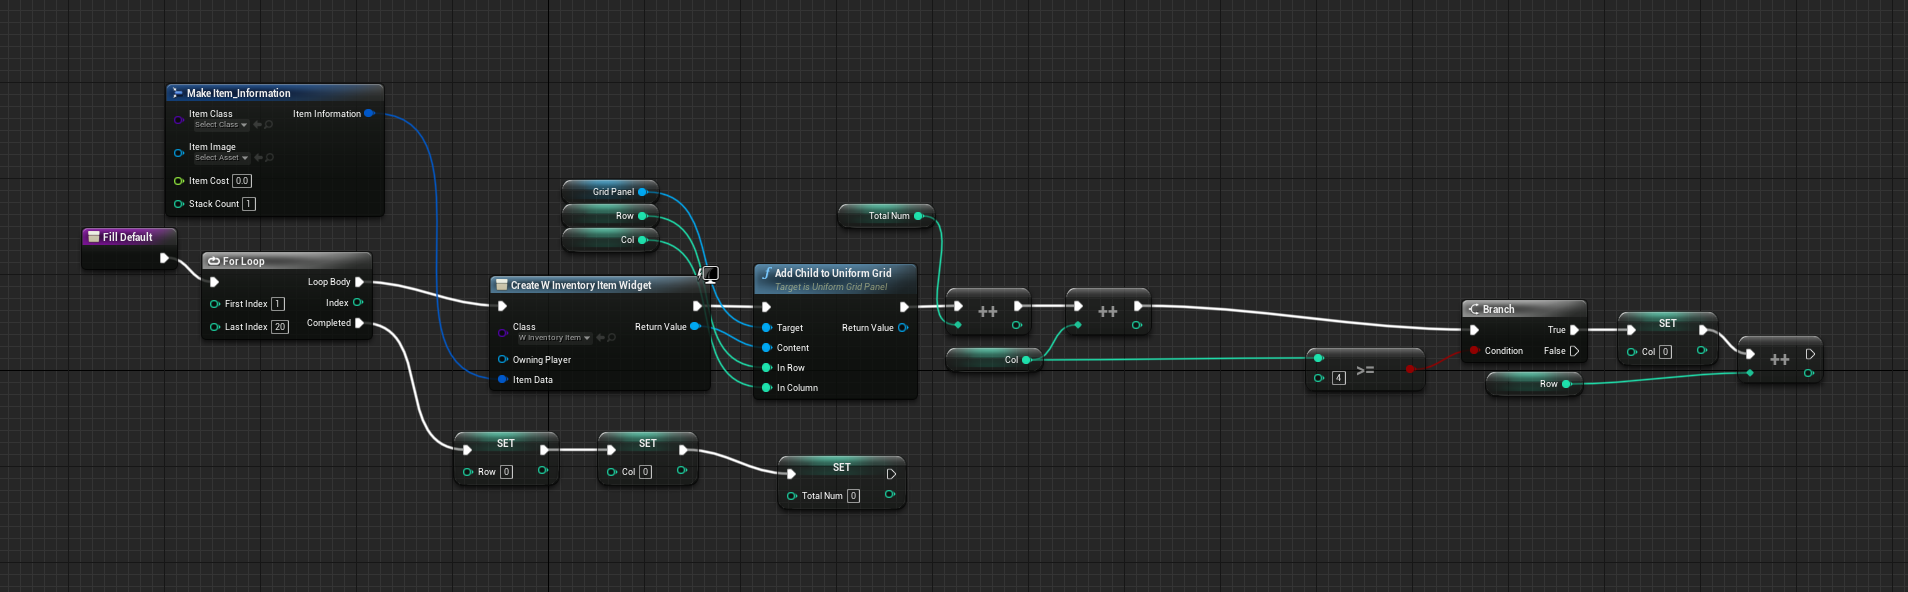
\includegraphics[scale=.3]{img/InventoryDefault.PNG}
    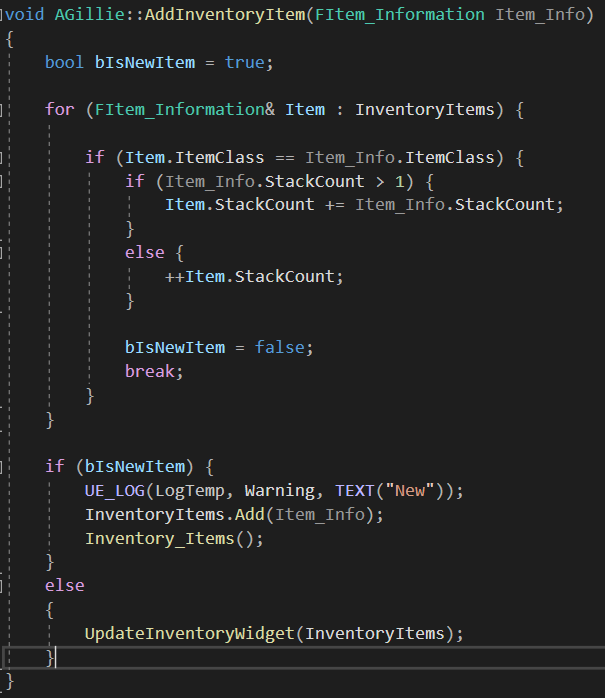
\includegraphics[scale=.3]{img/AddInventItem.PNG}
    \caption{Default Inventory and adding to inventory}
    \label{Default Inventory}
\end{figure}
The setup of inventory is done between both C++ code and blueprints. Using the Blueprints with the Widgets are easier to get it to work rather than using the C++ code as it is a little harder to connect everything together and has a chance of far more errors, So that is the reason behind using the blueprints for the most part. In the Player .Cpp file there is a function called \textbf{AddInventoryItem(FItem\_Information Item\_Info)} which takes a parameter of the struct. This function lets the player pick up the items and add them to the inventory with the combination of blueprints they will stack them by using this C++ code as shown above.
\begin{figure}[H]
    \centering
    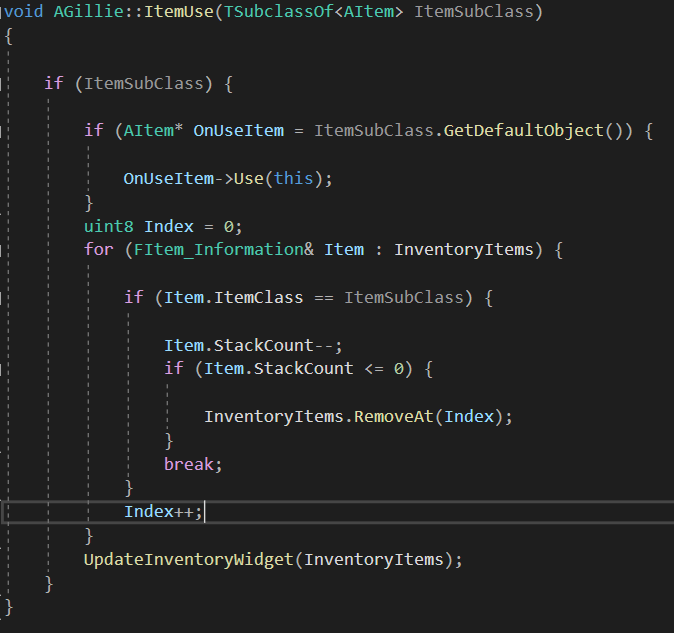
\includegraphics[scale=.4]{img/ItemUse.PNG}
    \caption{ItemUse Function}
    \label{ItemUse}
\end{figure}
In the player class there is a function called \textbf{ItemUse} which takes in a parameter of \textbf{TSubclassOf<AItem> ItemSubClass}. So with using the TSubclassOf this lets us create a subclass of AItem and then give it separate parameters and not have those assigned to any other item that we make off of the Item class. In the scope of this function it lets us use the item if needed and then also either decrements the count of the stack or if its the last item on the stack it will just remove it from the inventory. This operation is done within a for-each loop. And at the end of that operation there is another function called  \textbf{UpdateInventoryWidget} which takes \textbf{const TArray<FItem\_Information>\& NewInventoryItems} this is passed in an array that updates the inventory for the player and when an item is used it will take it of the stackcount and when it reaches zero it will remove it from the inventory and let some other item take that slot in its place.
\begin{figure}[H]
    \centering
    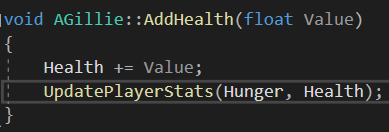
\includegraphics[scale=.6]{img/AddHealth.PNG}
    \caption{AddHealth Function}
    \label{HealthFunction}
\end{figure}
With the functions mentioned above the use item lets the player use items such as a health pack to heal themselves after fighting with the AI and taking damage to there HealthPoints. This was done by making a function \textbf{AddHealth(float Value)} the value is just like temp where it just gets passed in to do its update of the players health with every time the player calls the function from healing. There is a similar function called RemoveHunger which also takes a float as a parameter and does the same functionality as AddHealth.
\newline
\newline
\subsection{Attacks}
The next implementation that I did for the player was to set up the basics of the fighting and to get a Animation Montage which lets you group animations together and is really useful for the having a multiple amount of them together to make a moveset and not have the same attack always come up over and over again. 
\begin{figure}[H]
    \centering
    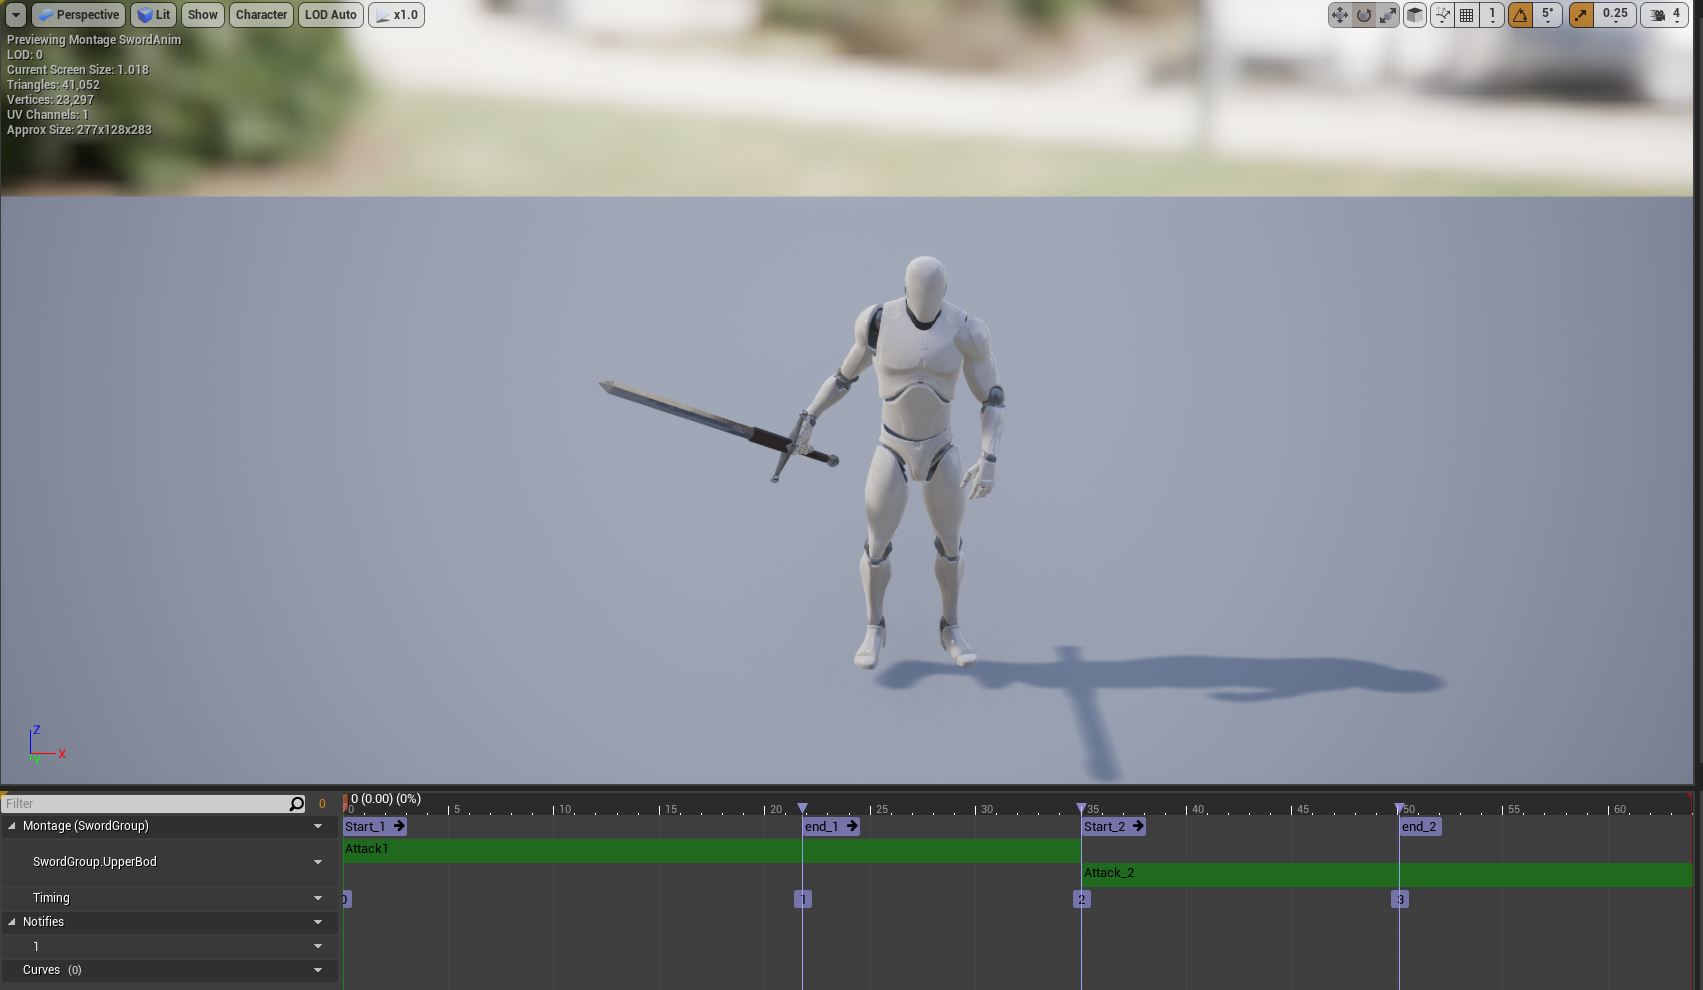
\includegraphics[scale=.3]{img/AnimationMontage.PNG}
    \caption{Player Attack Montage}
    \label{Attack Montage}
\end{figure}
These animations or attacks are set to be used by both pressing the alt + Mouse1 at the same time and this will call the function WeaponAttack calls a function from a class called \textbf{WeaponBase} called Slash. The function Slash lets the animations play and also lets the player cause damage to the player by calling the TakeDamage function which takes in 4 parameters each of these parameters are essential to causing damage to the AI when the SwordCollisionBox overlaps with an Actor. The first parameter is the amount of damage that is done to the Actor it collides with, the second is an event called FDamageEvent which lets a hit happen regardless of the type of hit that has been played. The third is a controller which can be passed as a nullptr as it will be the player who is doing the damage. And the last is the causer of the damage which you pass in \textbf{this} meaning the player character.
\begin{figure}[H]
    \centering
    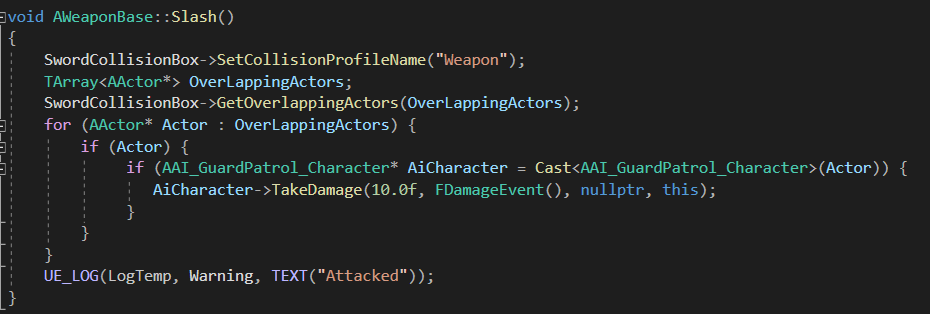
\includegraphics[scale=.4]{img/Slash.PNG}
    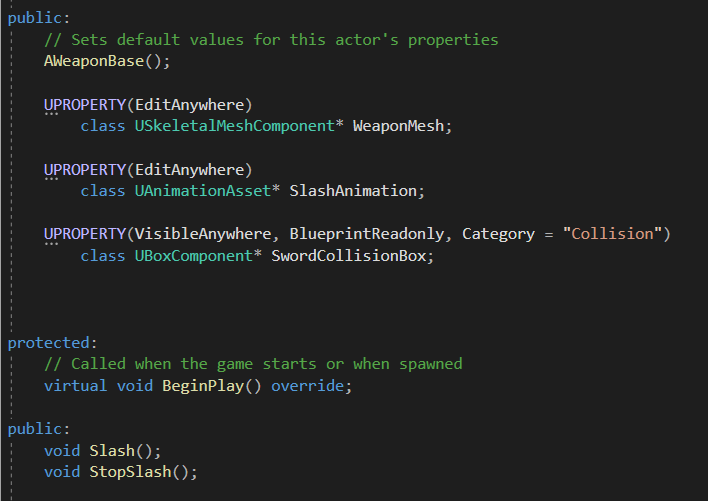
\includegraphics[scale=.4]{img/WeaponBaseH.PNG}
    \caption{Player Attack Montage}
    \label{Attack Montage}
\end{figure}
The WeaponBase is used to make all different types of weapons for both AI and Player. This takes in \textbf{USkeletalMeshComponent} and lets you assign any kind of weapon that you would like to it. This is then assigned to Rootcomponent which lets us attach it to the player. And then for the weapon to be able to apply damage to others in the world we attach a \textbf{UBoxComponent} so this can be set to be the collision on the blade and inflect the damage on others. But the damage is only turned on when you use the attack buttons and as soon as those attacks are done they are turned off so they cannot just cause harm to anything while walking around the world.
\begin{figure}[H]
    \centering
    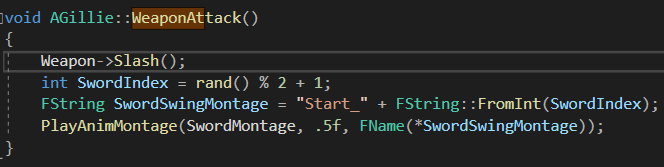
\includegraphics[scale=.6]{img/WeaponAttack.PNG}
    \caption{Player Weapon Attack}
    \label{WeaponAttack}
\end{figure}
The \textbf{WeaponAttack} function also has a animation montage within it which lets 2 different animations be played if you use 1 or 2 mouse clicks. It uses a rand() function to run either animation at the start of every attack. But there is an issue with this if you have 3 animations and have it set to \textbf{SwordIndex = rand() \% 2 + 1;} then the Editor of Unreal Engine will crash and not give you an error as it thinks that there should be 3 animations to be picked from.
\subsection{AI \& NPCS}
With setting up of the AI \& NPCS I used a Character and a AI Controller. The character was picked instead of a pawn as a pawn is just a physical representation, as to where the character can do what a pawn can do and more. The character comes with some basic movement and can be set up a little bit easier than the pawn also which would save workarounds such as using Behavior Tree which is very like a state machine and takes away from learning the C++ language of coding so. The Behaviour tree is then used with a Blackboard which becomes the brain of the AI and then combines with blueprints to make up the AI. But I decided to go down the pure C++ route and really get to know the C++ language this is where the C++ classes of the Character and the AI Controller come in to play.
\begin{figure}[H]
    \centering
    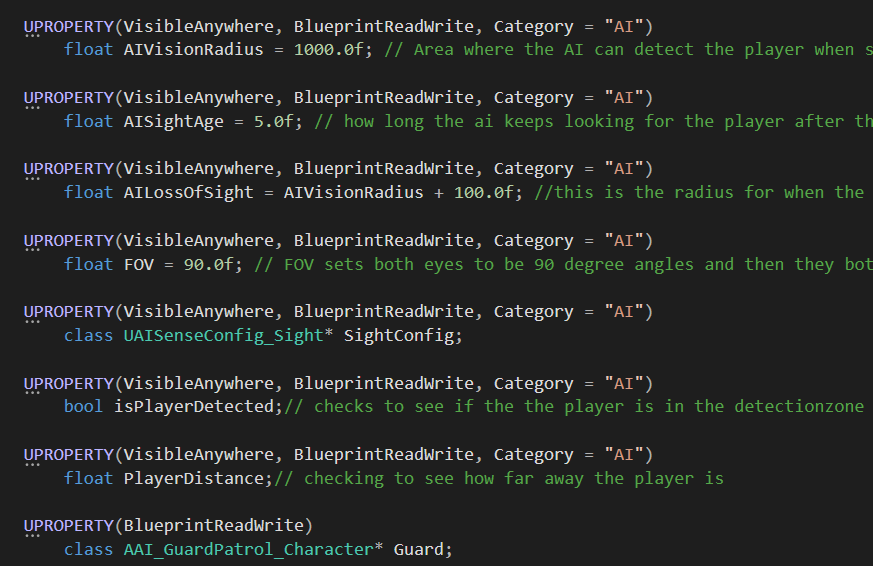
\includegraphics[scale=.5]{img/AIController.PNG}
    \caption{AIController}
    \label{AiController}
\end{figure}
The AI Controller is the brain of the AI that is being coded up and this is where it almost becomes life like as it takes in a number of parameters or UPROPERTYS which they are called in Unreal Engine. Each of these properties are doing something to detect and see if the player is friendly or an enemy and how this is done is by using a library called \textbf{Perception/AIPerceptionComponent.h} which lets the AI use the senses of Sight, Sound or Touch. For this project I decided to use the one and that was sight. So for setting up the sight you give a Vision Radius which is a circle around the AI head and you can make it as big as you like so if you wanted to have an AI using Binoculars or a telescope the radius would be far bigger. 
You also have a Field of Vision(FOV) which acts like peripheral vision and once the player or enemy walks into that FOV they will either attack or just let you do your thing and let you be. And like what is said above with having AI using Binoculars or a telescope the FOV would be smaller and harder to spot the player/ enemy.
There is also a distance that you can set for the AI to lose sight of you which then activates a timer and will go to your last known position until that timer hits 0 and when it is at 0 they will go back to what they were doing such as standing guard or patrolling. All of this work is done in the following functions that will be highlighted in bold the first of which takes an array of Actors \textbf{OnPawnDetected(const TArray<AActor*>\& DetectedPawns)}. When this function is called/activated it will go through a for loop to see how many there is detected and then will make a bool isPlayerDetected turn to true and sends this to another and will attack if it not a friend.
\begin{figure}[H]
    \centering
    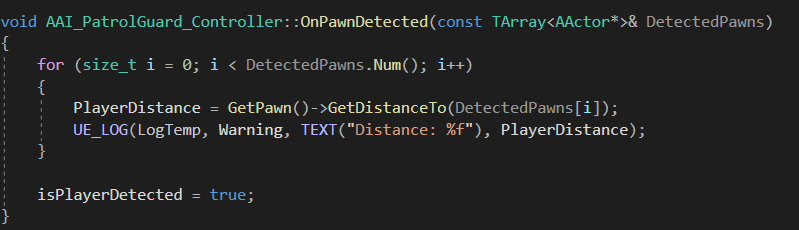
\includegraphics[scale=.5]{img/Detected.PNG}
    \caption{Detecting other Players and AI}
    \label{Detection}
\end{figure}
The next then is an overridden function \textbf{GetTeamAttitudeTowards} which takes a parameter of AActor. This function works in unison to the OnPawnDetected. The GetTeamAttitudeTowards function is an overridden function that takes a parameter of AActor. This function works very similar to how a decision tree works but a more refined version of it as it only has a small number of checks to do such as checking to see if the player or other AI is neutral, friendly or an enemy and with these they then check to see the id of the which it has detected and if the id does not match theirs then they will enter attack mode. The only way if you can not be attacked is if your id is the same or if your id matches that of the neutral AI. But just because they are neutral may not stop them attacking them.
\begin{figure}[H]
    \centering
    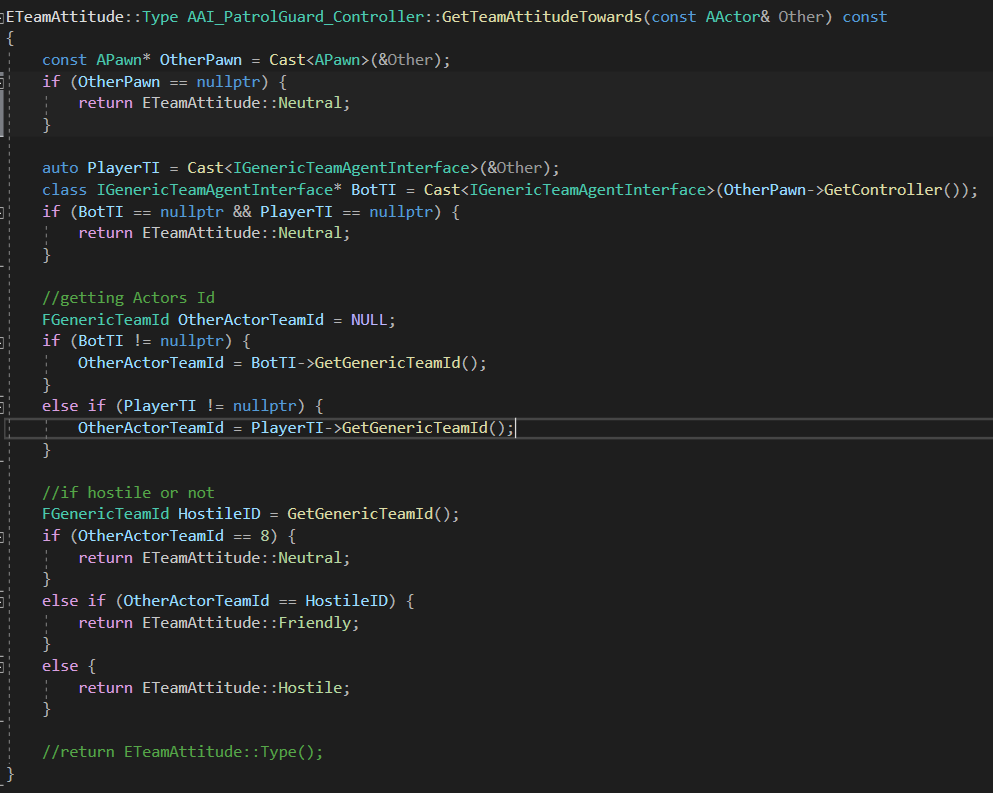
\includegraphics[scale=.4]{img/Team.PNG}
    \caption{GetTeamAttitudeTowards Function}
    \label{GetTeamAttitudeTowards}
\end{figure}
The next thing we have is the Tick function. This function auto generated and is called every frame and makes the character class move about if so. The Tick function is like the heart of the class. In the Tick function the control of the AI is setup and it controls if it is going to each way-point that it has been assigned to go visit. Also within the function it holds the code to inflict damage to the player as it makes a call to the WeaponBase class and calls the AttackPlayer Function was mentioned in the Attacks Subsection above.
\begin{figure}[H]
    \centering
    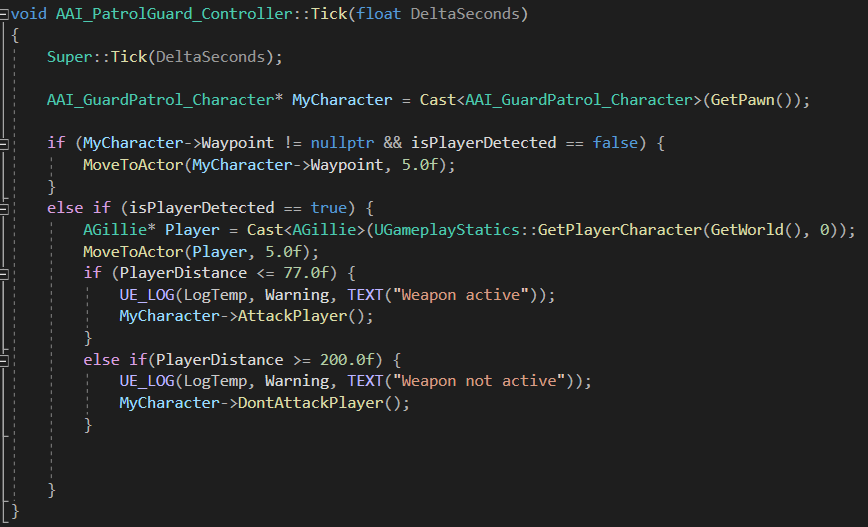
\includegraphics[scale=.4]{img/AITick.PNG}
    \caption{AI Tick Function}
    \label{Ai Tick}
\end{figure}
The first time of writing this waypoint class and having the AI use it was just an array of waypoints that would just be an infinite loop of the using a for loop and it would always start at one and then just increment through the loop until it got to the last one int he array and then they would just stand in that position and that would be the end of the movement so to keep the AI moving about the map you would need it to have 100s of them in the array and this would take up loads of space in memory which is not good. So I went and did some research on how to get the AI on how to move around the map in a better way. And the way I decided the AI moves about the map is by been told to go to a Waypoint that is made from the Actor class in Unreal Engine. The Waypoint class is given a UFUNCTION called \textbf{OnPlayerEnter} and is passed six parameters, the OnPlayerEnter function works with the UBoxComponent. It is then attached to a BoxComponent which then acts as trigger which will update the AI on the waypoint it needs to visit next and this is then the previous one is not stored anywhere in the AI only in the waypoint that tells it to visit the next one.
\begin{figure}[H]
    \centering
    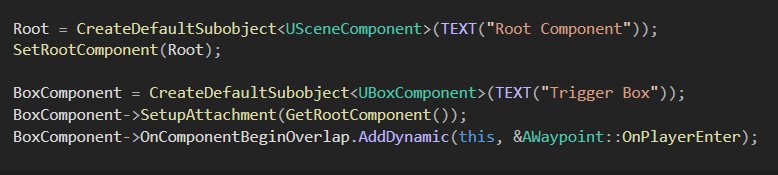
\includegraphics[scale=.5]{img/WaypointTrigger.PNG}
    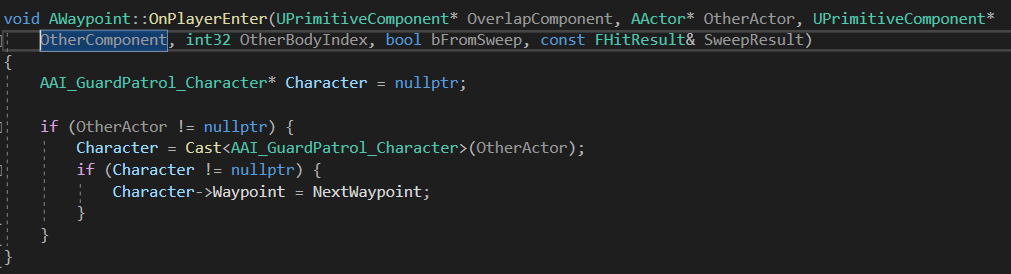
\includegraphics[scale=.5]{img/PlayerEnter.PNG}
    \caption{AI Waypoint}
    \label{AI Waypoint}
\end{figure}
\subsection{AI Attacks \& Damage}
The AI has a \textbf{AttackPlayer} function within the Character class that does the attack animation to the player or enemies. In this class the AI gets the mesh or how it should look if given a skin/asset that you like it to look like. The class is given a UPROPERTY that is a UAnimMontage which lets us you manipulate how it is executed in the game and the timings of it such as how fast the animation is played and set the collision presets for the weapon that the AI is wielding, so in the attack player it is given the preset of "weapon" and this lets the sword in this in instance deal damage to anything that is not the owner as shown in the image below. 
\begin{figure}[H]
    \centering
    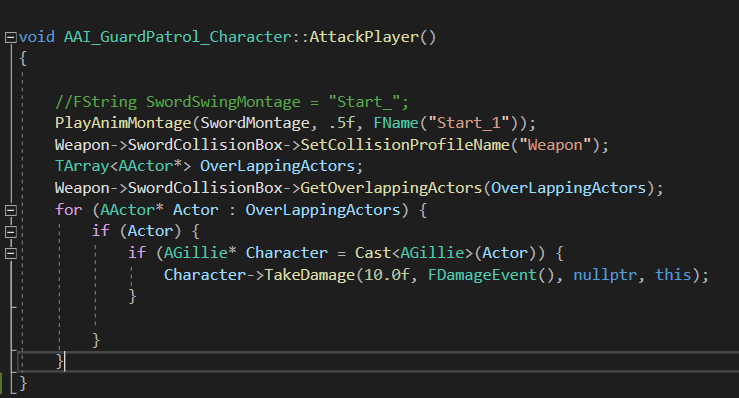
\includegraphics[scale=.5]{img/AttackPlayer.PNG}
    \caption{Attacking the player}
    \label{AI Waypoint}
\end{figure}
The Sword is attached to the AI by going into the skeleton of the character and adding a socket and then attacking the sword to the socket with the name "right\_fist\_col" to make it look like the AI is holding the weapon as shown below.
\begin{figure}[H]
    \centering
    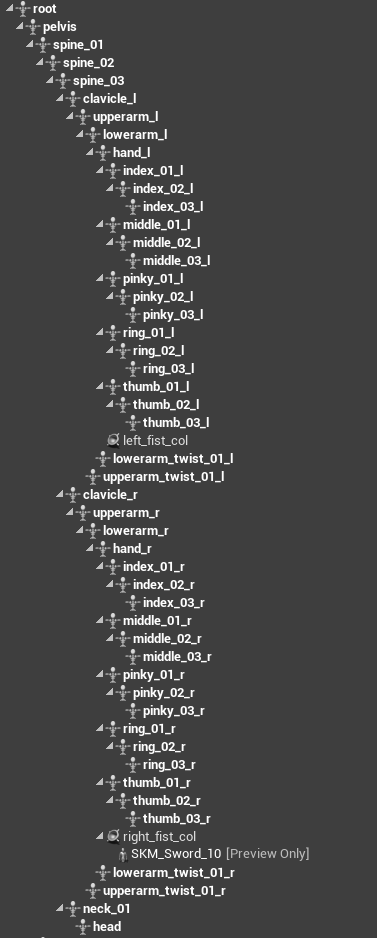
\includegraphics[scale=.3]{img/Skeleton.PNG}
    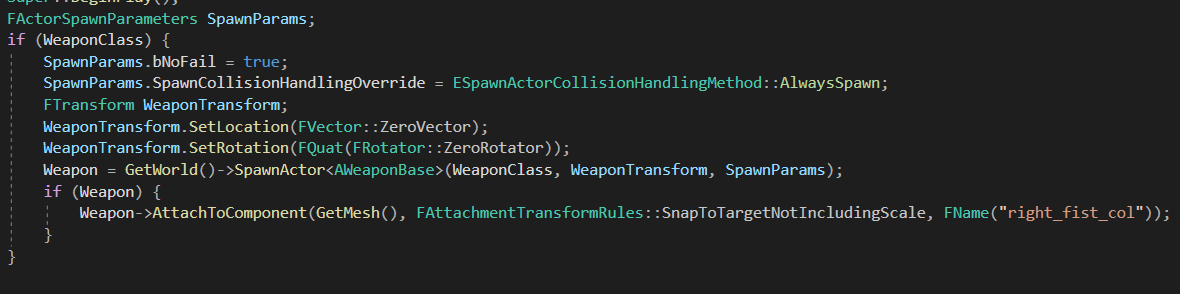
\includegraphics[scale=.3]{img/AIAttachSword.PNG}
    \caption{Skeleton and Attaching Sword}
    \label{Skeleton}
\end{figure}
This is is all done in the Tick function again as we need the sword to stay hand for every frame while the AI is walking around. Another function in this class is \textbf{DontAttackPlayer} that calls a function from the WeaponBase class that turns off all collisions and wont be able to inflict damage to the player or AI when just walking past. The final function that is in this class is TakeDamage that is also on the Player and is the same as what has been mentioned above.
\subsection{Level Design}
\begin{figure}[H]
    \centering
    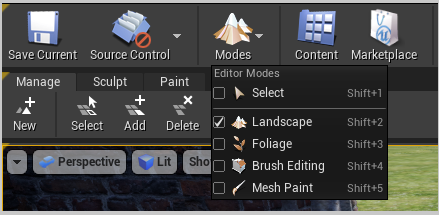
\includegraphics[scale=.7]{img/Landscape.PNG}
    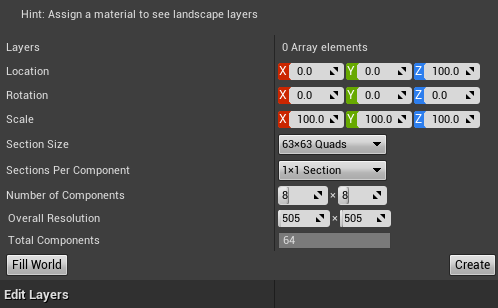
\includegraphics[scale=.6]{img/ManageLandscape.PNG}
    \caption{Level Design}
    \label{Level Design}
\end{figure}
Working on the level design which was setting up the map of the area where the player can go and move about the world. When you first start to the level design you have to click on New under manage you will be given a choice on what size landscape with the smallest being 7x7 and the largest at 255x255 and the middle at 63x63 which was chosen for this game as it was only meant to be a demo or prologue on what can be done in the unreal engine without any prior knowledge of the engine. The 63x63 is in the range of what 2km x 2km would be in real work units. This is also quite big for the world that is need for what has been done in this project, as it has one main town, two small villages and a little cave that players can enter if they come across it. With doing the level design you can use ten different tools to create what is need in the level, so to create humps and hollows you could use the first tool that is selected which is just sculpting but from using the tools and finding what works best for this is Erosion tool that lets you both raise and lower at the same time and this makes the lay of the land look like it would in real life and not just hills that are completely smooth with little to no details on them.
\begin{figure}[H]
    \centering
    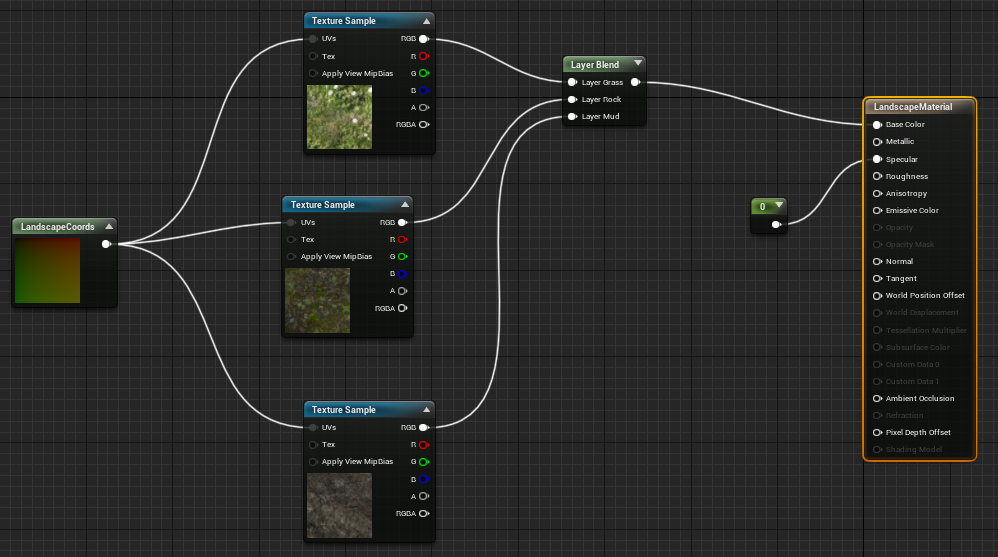
\includegraphics[scale=.5]{img/LandscapeMat.PNG}
    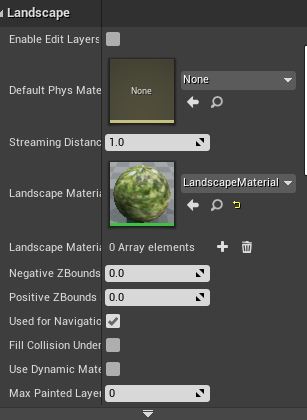
\includegraphics[scale=.5]{img/LScape.PNG}
    \caption{Landscape Material}
    \label{Level Design}
\end{figure}
To get the world to look like there is something on the ground and to not have it just there as grey matter you need create a landscape material that will let you to make the ground look how you please such as a grass,rock,mud or any other earth looking type you would like it to be. The landscape material adds so much to the world and how it looks to the eye of the player even tho it looks like a layer of paint but for something so small it does something so huge. In the image above you can see that there is 3 textures within the material this lets the Dev pick from which colour they want when they are painting the ground after this has been added to the Landscape as shown is the image above. When painting you can only use those 3 colours but you can add more into the landscape material and then you can go ahead and paint with that colour then. 
\begin{figure}[H]
    \centering
    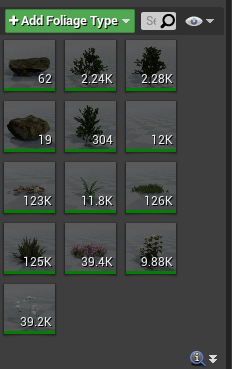
\includegraphics[scale=.7]{img/Foliage.PNG}
    \caption{Foliage}
    \label{Level Design}
\end{figure}
To add some more detail than just painting the landscape and using the landscape tools you can add foliage such as rocks, trees, flowers, grass etc all of these combined in the right way can really bring a game to life with it being more than just being baron wasteland.
\begin{figure}[H]
    \centering
    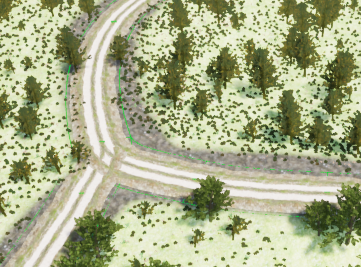
\includegraphics[scale=.5]{img/Spline.PNG}
    \caption{Foliage}
    \label{Spline}
\end{figure}
To make roads or path ways you can use a thing called a spline. Splines are something that you can keep adding to and make it as long as you like and can be manipulated into how normal roads and paths would look in real life which is far easier than having to lay then down one by one. If you are trying to make a road that has multiple turns and and some hills and dips splines will also make the lay of the to the way you want it without having to build the land to it. This proves very useful for making paths into a mountainous area of to the top of a hill with a dead-end. Splines are also used on the likes of rivers or it can even be used to setup wiring or plumbing in a building.
\newline
\par\nobreak \textbf{Blender}
I also had to learn a small bit of Blender, Which is a tool to create assets for games. In Blender I had to create the door that was mentioned above earlier. I had to create two timelines, one for Opening of the door and Closing of the door this proved to be a little tricky to workout and get right as it was something that I wasn't used to doing. But the Opening and Closing fit into two property's(\textbf{UPROPERTY}) which is then called a UAnimateAsset. With blender this also makes the mesh to add collision with the player so the player cant run through without having to use the open or close function.
\begin{figure}[H]
    \centering
    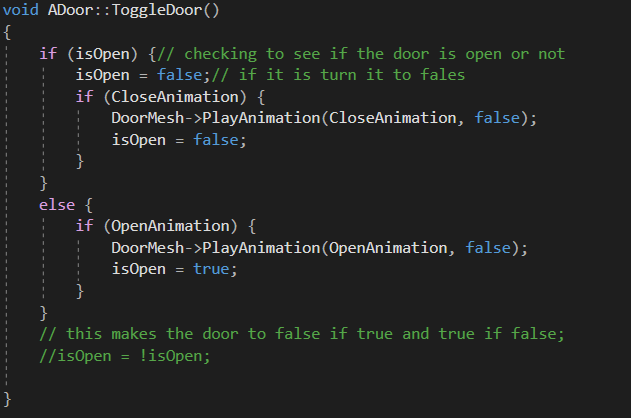
\includegraphics[scale=.4]{img/Door.PNG}
    \caption{Door code}
    \label{Door}
\end{figure}
When making the door using blender and this was most likely the hardest thing to do in the whole project as it was something totally out of the scope that I would have ever learned and know and this proved to be somewhat of the second hardest challenge that I came across while doing this project as it was difficult to find a the right material that actually showed how to make a door. There was one video series I found on YouTube that let me learn how to use the very basics of Blender and by the basics I mean by making a rectangle work like a door. This was such a reward to actually see working after I had finished it as I also had to make two animations for it in blender using timelines and the only experience I had with timelines before this was in a assignment we had done in the previous semester in Mobile game development where we had to make a game on a timeline, so having that little bit of experience in using them help me a lot on how to get the to work. The timelines were for opening and closing the doors. This also entailed the use of the C++ scripts as it took in 2 animations would play each animation if a bool called isOpen was set to true and then if false it would let the player close it.
\chapter{System Evaluation}
\subsection{Limitations or Opportuni-ties}
The Opportuni-ties of this project for me was to see if I was able to go and learn a new programming language that would challenge me and also something that would be able to really show of how good that language is how much of it was able to learn in the span of the college year without someone holding my hand along the way. The idea I went for was learning to make a game in the Unreal Engine and this really showed the power and speed of the C++ language which with nearly every time I did or done something new in the programming language it blew me away time and time again and this was just like the first time I was learning to write simple programs in Java. This was a whole different ball game as it was doing something completely different in trying to make an open world game with having a player to do as they like and also be able to fight an AI that was well written and not just something at will run up to the player and let the player attack and kill it. The AI that I learned to write code for while doing this project was some of the most impressive stuff I have learned while in my 4 years as a college student. One thing that I wished I had added into my game was a save and load feature but I focused to much on other aspects of the project that were a little more complex and trying to make everything that little bit better. But that is something that I have learned while doing this project is to get something and then make it better after you have all the main features of it done.
\newline
\newline
With all that is said above one of the limitations is testing and running automated tests in the background while I was doing work to something else. And with that I was just testing everything that was done myself. So if something was added to the player like to attack with a sword I would test that myself instead of using the testing capabilities that are in the Unreal Engine. This is something that I will learn to use moving forward while I continue to add to this i will do more tests even tho this will be more time consuming it would benefit the project and myself in the long run becasue of the time spent on writing the tests would then be made up down the road for me actually coding and not have to play test and make sure it does what I need as to where I could have a few simple tests doing this and I could be using the time where tests are being done doing something to the project itself.

\chapter{Conclusion}
The one thing I set out while doing this project was to be able to step out of my comfort zone and learn something new with a programming language. With learning C++ in the college year I know how to use one of the most powerful/fastest programming languages that is out there. With undertaking this project I have also learned better coding aspects such as learning that more is never better as is could get messy very fast as it can lead to mistakes and things can look like spaghetti code which is something that is extremely bad. Learning that less code can do a lot more than just churning out massive blocks of code is far more productive and you learn more with the small amounts of code. I also learned that GitHub is your best friend when doing a project like this when you have done some code and it seems to break everything you can also just go back to the last commit and that is what I learned from this project the HARD way as I started I was just committing massive amounts of code and then if something went wrong and had to role back all that work was wasted. As I said above that small amounts of code are better, well committing those small bits of code are the things that make or break you as a software developer because if you only have to go back one previous commit of a small code block you dont have to spend half the day redoing all the work again and not get frustrated at something that your making and just leaving it out of frustration.
\newline
\newline
I have also that game design is harder that I had first thought but it is something that I have really enjoyed, I always said it cant be that hard to get x working for the big name game devs that are out there but doing this project it has really humbled me as I now know how hard it is to get some of this stuff working and have it all come together and when it eventually does it is something else. The AI was one of the hardest and most enjoyable bit of coding I have done as it was so good to see them first have the halo around there head and then eventually seeing that the AI can not just detect the player via sight but also by sound and touch which is something incredible. And with learning everything in the project that I have I still want to continue learning more about what it can do for the game, so hopefully in a short while down the road I will continue committing to the repo and keep the ball rolling on the game. 


